%%%%%%%%%%%%%%%%%%%%%%%%%%%%%%%%%%%%%%%%%
% Capture the flag Writeup Template. 
% LaTeX Template
% Version 1.0 
%
% This template has been downloaded from:
% http://www.latextemplates.com
%
% Original authors:
% Hector F. Jimenez S. <hfjimenez@utp.edu.co>
% Pereira Security Team 2013.
% License:
% CC BY-NC-SA 3.0 (http://creativecommons.org/licenses/by-nc-sa/3.0/)
%
%
%----------------------------------------------------------------------------------------
%	PACKAGES AND OTHER DOCUMENT CONFIGURATIONS
%----------------------------------------------------------------------------------------
\documentclass[a4paper]{article}
\usepackage[spanish]{babel}
\usepackage[utf8x]{inputenc}
\usepackage[T1]{fontenc}
\usepackage{amsmath}	
\usepackage{graphicx}
\usepackage{url}
\usepackage{color}
\usepackage{hyperref}
\hypersetup{
    colorlinks,
    citecolor=black,
    filecolor=black,
    linkcolor=black,
    urlcolor=black
}
\usepackage[export]{adjustbox}
\usepackage{geometry}
 \geometry{
 a4paper,
 total={210mm,297mm},
 	left=30mm,
 	right=20mm,
 	top=20mm,
 	bottom=20mm,
 	bindingoffset=0mm
 }
 

\title{Titulo del Reto }
\author{Correo El\'ectronico \\Nombre}
\begin{document}
\begin{titlepage} 				
\begin{center}	  				
\vfill
\line(1,0){250}\\ 				%Lineas Horizontales.Nombre de Desafio y Reto
\huge\textbf{Desafio}\\	
\large{Nombre}\\
\large\texttt{@Twitter}\\
\line(1,0){250}\\
\large{Pereira Security Team}
\end{center}
\vspace{4em}
\centerline{
\includegraphics[width=\textwidth]{barcampse_2013_logo-_281_29}} 			%Logo del Evento
\vspace{7em}																			%Espacio entre imagen e imagen
\centerline{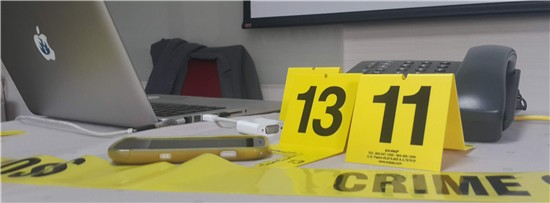
\includegraphics[width=\textwidth]{afr}} 									%Logo del Reto


\vspace*{\stretch{2.0}}
\end{titlepage}
																			%Pagina En blanco
\clearpage
    \thispagestyle{empty}
    \phantom{a}
    \vfill
    \begin{center}Pagina Dejada Intencionalmente en Blanco\end{center}
    \vfill
\newpage
\tableofcontents
\newpage
\clearpage
%\maketitle
\begin{abstract}
Un Resumen Rapido para Esta Seccion.
\end{abstract}
\section{Introducci\'on}
Descripcion del Reto.

\section{Resumen Ejecutivo}Si es requerido de lo Contrario Borre Esta seccion Resumen Ejecutivo:\textit{Breve análisis de los aspectos más importantes del proyecto,El resumen ejecutivo es una s\'intesis de los puntos más importantes que conforman el reporte no siempre se pide pero si se exige pongalo aqui.El objetivo que se persigue con la elaboración de un resumen ejecutivo, es que el lector tenga una visión general del reto en general, así como que logre una comprensión e interés en el reto, y en seguir leyendo el resto de las partes que conforman el plan.}
\section{Solucion Retos \label{SolRet}}
\subsection{Reto1}
No olvide Incluir Imagenes.
%http://www.laqee.unal.edu.co/tex-archive/info/epslatex/english/epslatex.pdf
%\begin{figure}
%  \centering
%    \includegraphics{grafico}
%  \caption{Mi Figura}
%  \label{fig:ejemplo}
%\end{figure}

\subsection{Reto2}
No olvide Incluir Imagenes.
\subsection{Reton}
No olvide Incluir Imagenes.
\clearpage
\newpage
%Toolset.
\section{Herramientas \label{Herramientas}}
\begin{itemize}
\item \href{http://virtualbox.org}{Virtualbox}
\item \href{www.wireshark.org}{Wireshark}
\item \href{www.wireshark.org}{Terminal Based Wireshark}
\item \href{http://www.gnu.org/software/coreutils/}{Coreutils}
\item \href{http://www.secdev.org/projects/scapy/}{Scapy}
\item \href{http://www.chiark.greenend.org.uk/~sgtatham/putty/}{PuTTY}
\clearpage
\newpage
\section{Adjuntos}
Archivos Adjuntos: Scripts, Pruebas\ldots etc 
\clearpage
\newpage
\section{Agradecimientos}
Agradecimientos en esta seccion \href{http://www.ejemplourl.org}{Ejemplo URL} 

\end{itemize}
\end{document}
